Having obtained a final force field, the resulting model should always be
assessed and validated before use in molecular simulation. We divide this
topic into two sections -- sanity checks and validation -- to distinguish
between tests that can be performed via visual inspection of the fits compared
to those that require additional computations.

\begin{subsection}{Sanity Checks}

\begin{paragraph}{Visualization}

Once the \pointer code has been successfully run, the resulting force fields
should always be visualized, possibly with the aid of the included
visualization scripts:

\begin{lstlisting}
plot_compare_sapt_components.py -p <file_prefix> -s <file_suffix>'.dat' --display
plot_sapt_component_errors.py <file_prefix> <file_suffix>'.dat' --display
\end{lstlisting}

where additional visualization options are available by inserting the \verb|-h|
flag into the function call for either script. Such visualizations are shown,
using the pyridine dimer as an example, in
\cref{fig:pointer-pyridine_fits,fig:pointer-pyridine_errors}, and additional
visuals for water and other molecules are shown in \cref{sec:mastiff-fits}.

% \begin{landscape}
\begin{figure}
\centering
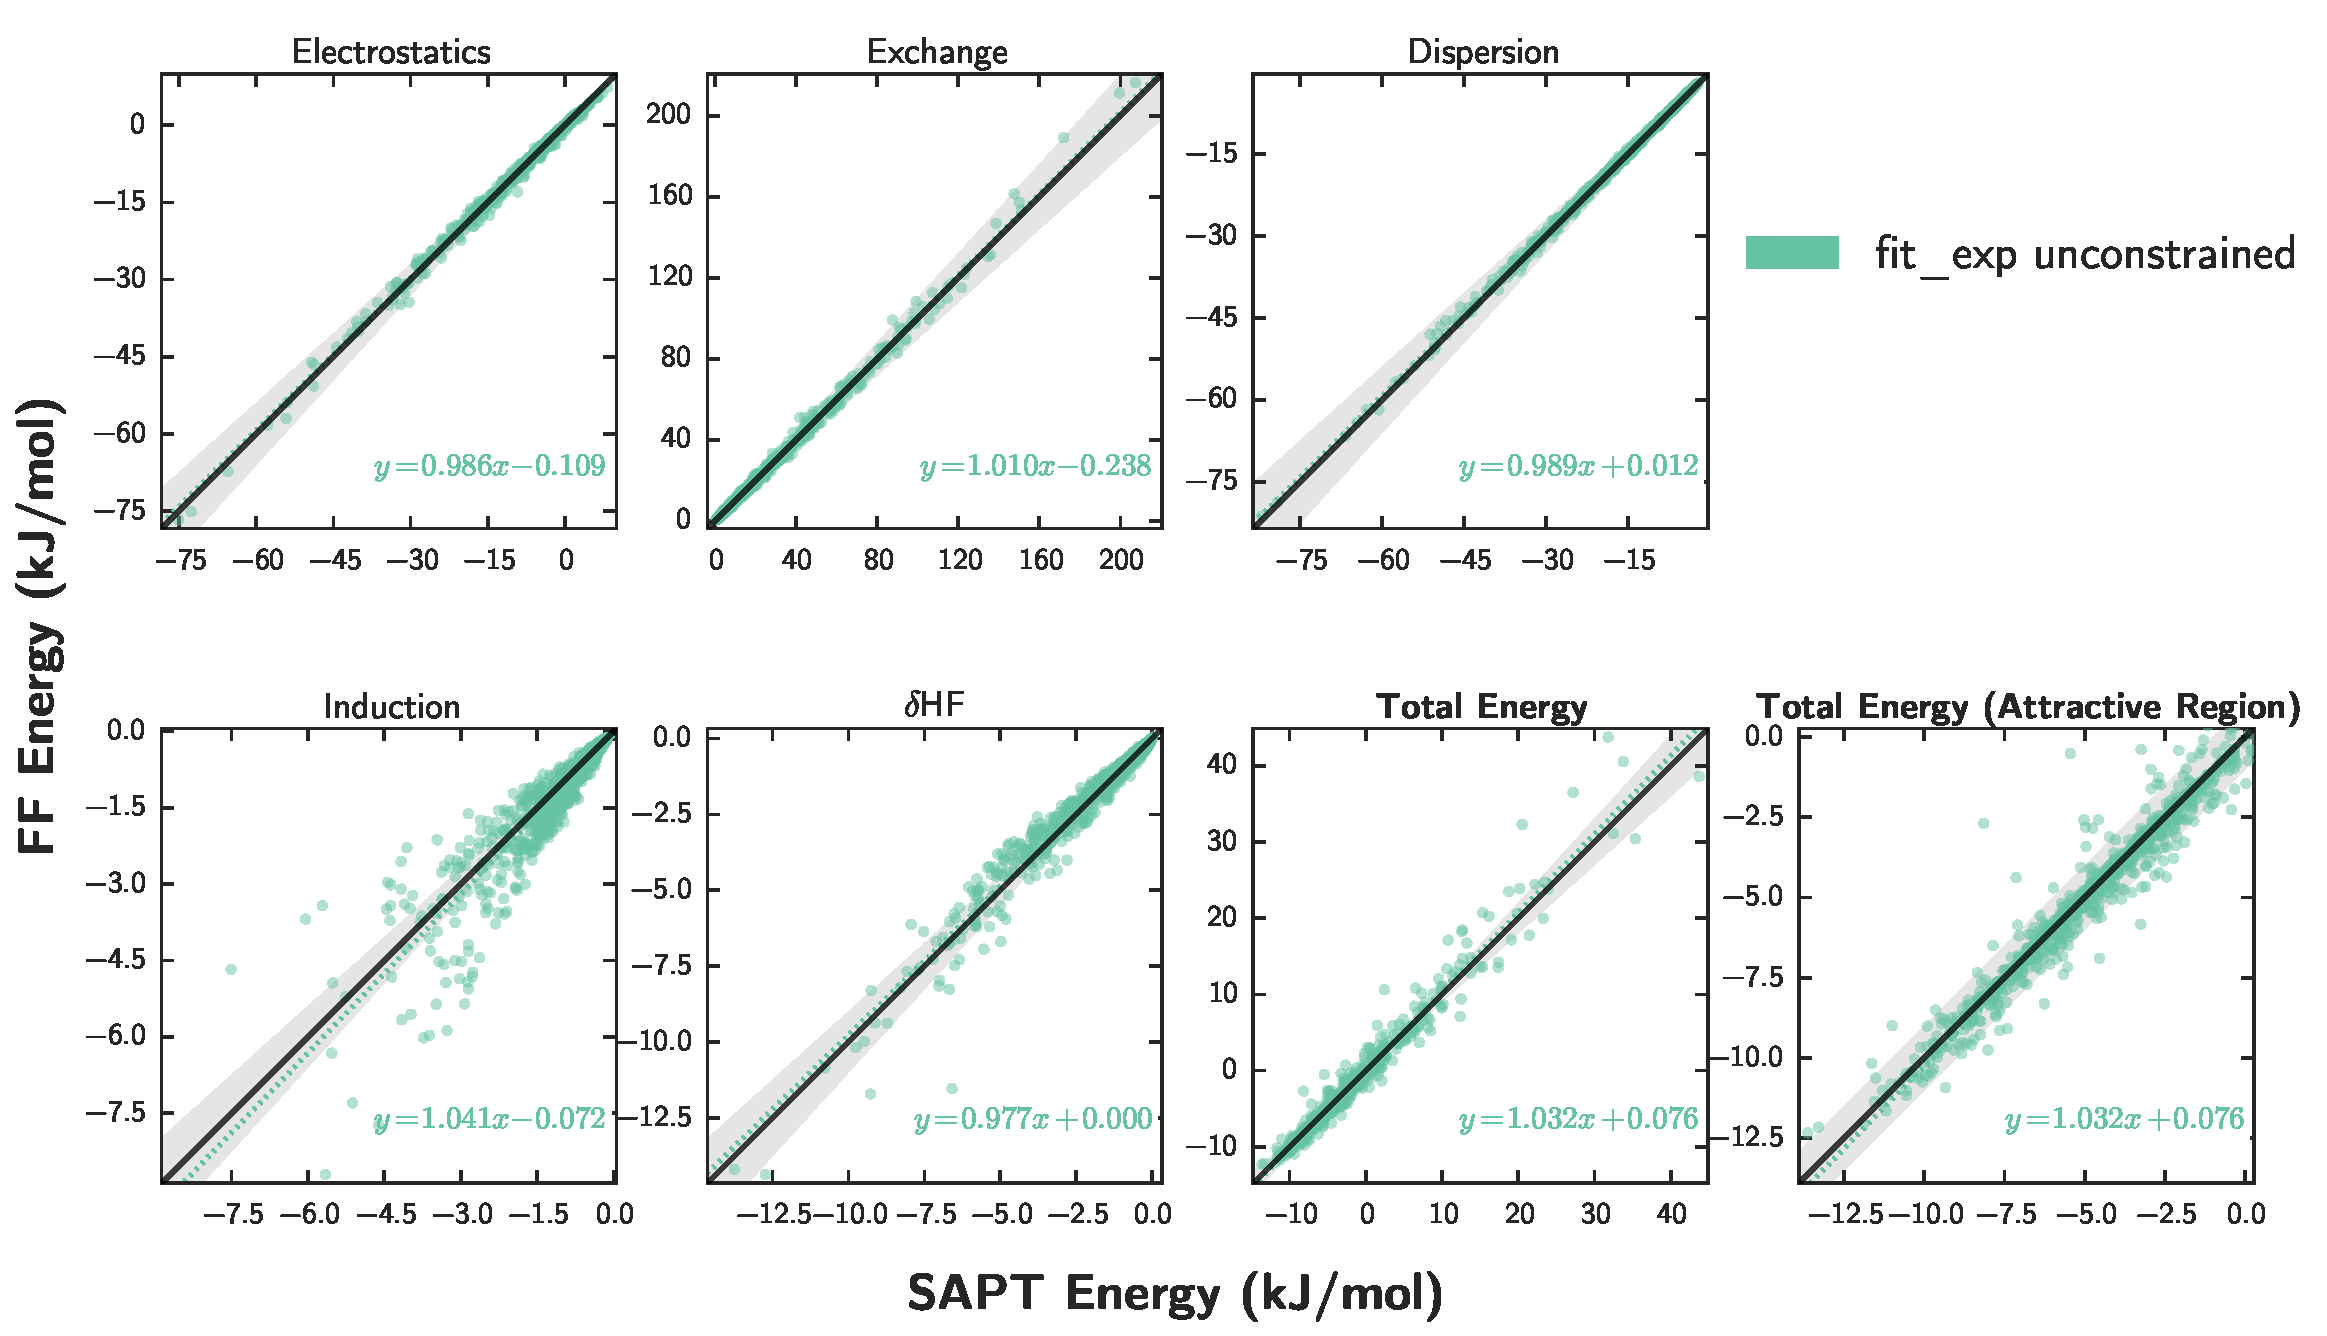
\includegraphics[width=\textwidth]{pointer/pyridine/sapt_comparison.pdf}
\caption[Comparison with the pyridine dimer]
{The pyridine dimer}
\label{fig:pointer-pyridine_fits}
\end{figure}

\begin{figure}
\centering
\fbox{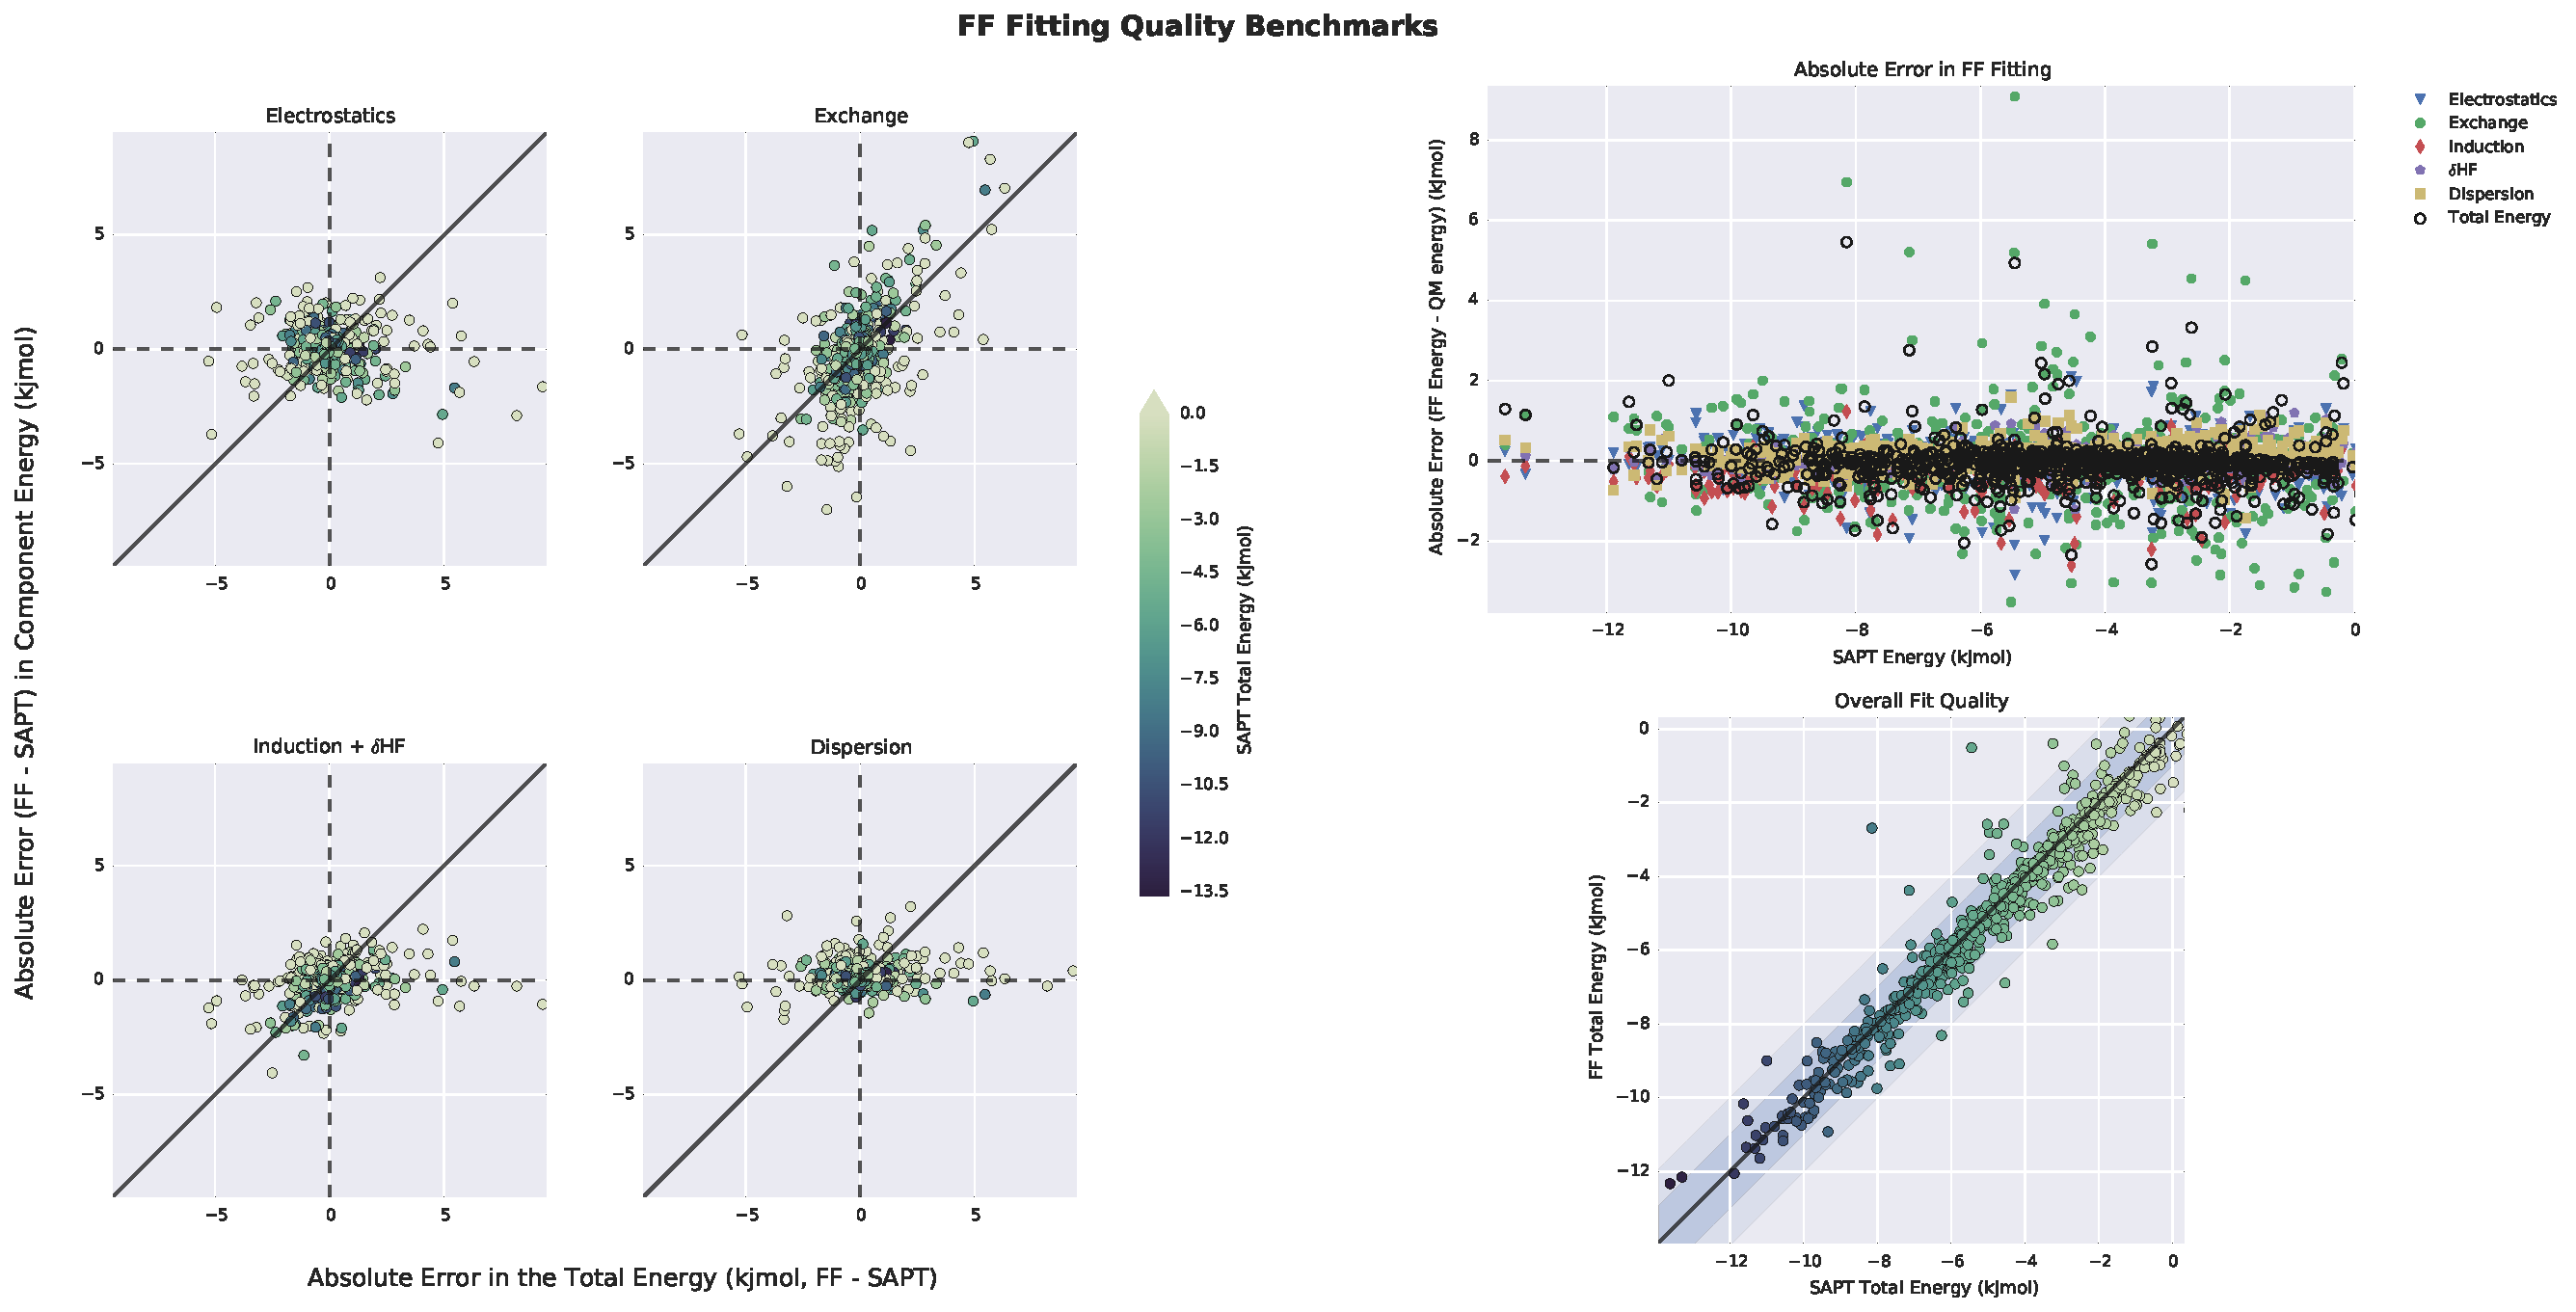
\includegraphics[width=\textwidth]{pointer/pyridine/fit_exp_sapt_errors.pdf}}
\caption[Errors with the pyridine dimer]
{The pyridine dimer errors}
\label{fig:pointer-pyridine_errors}
\end{figure}
% \end{landscape}

\begin{figure}
\centering
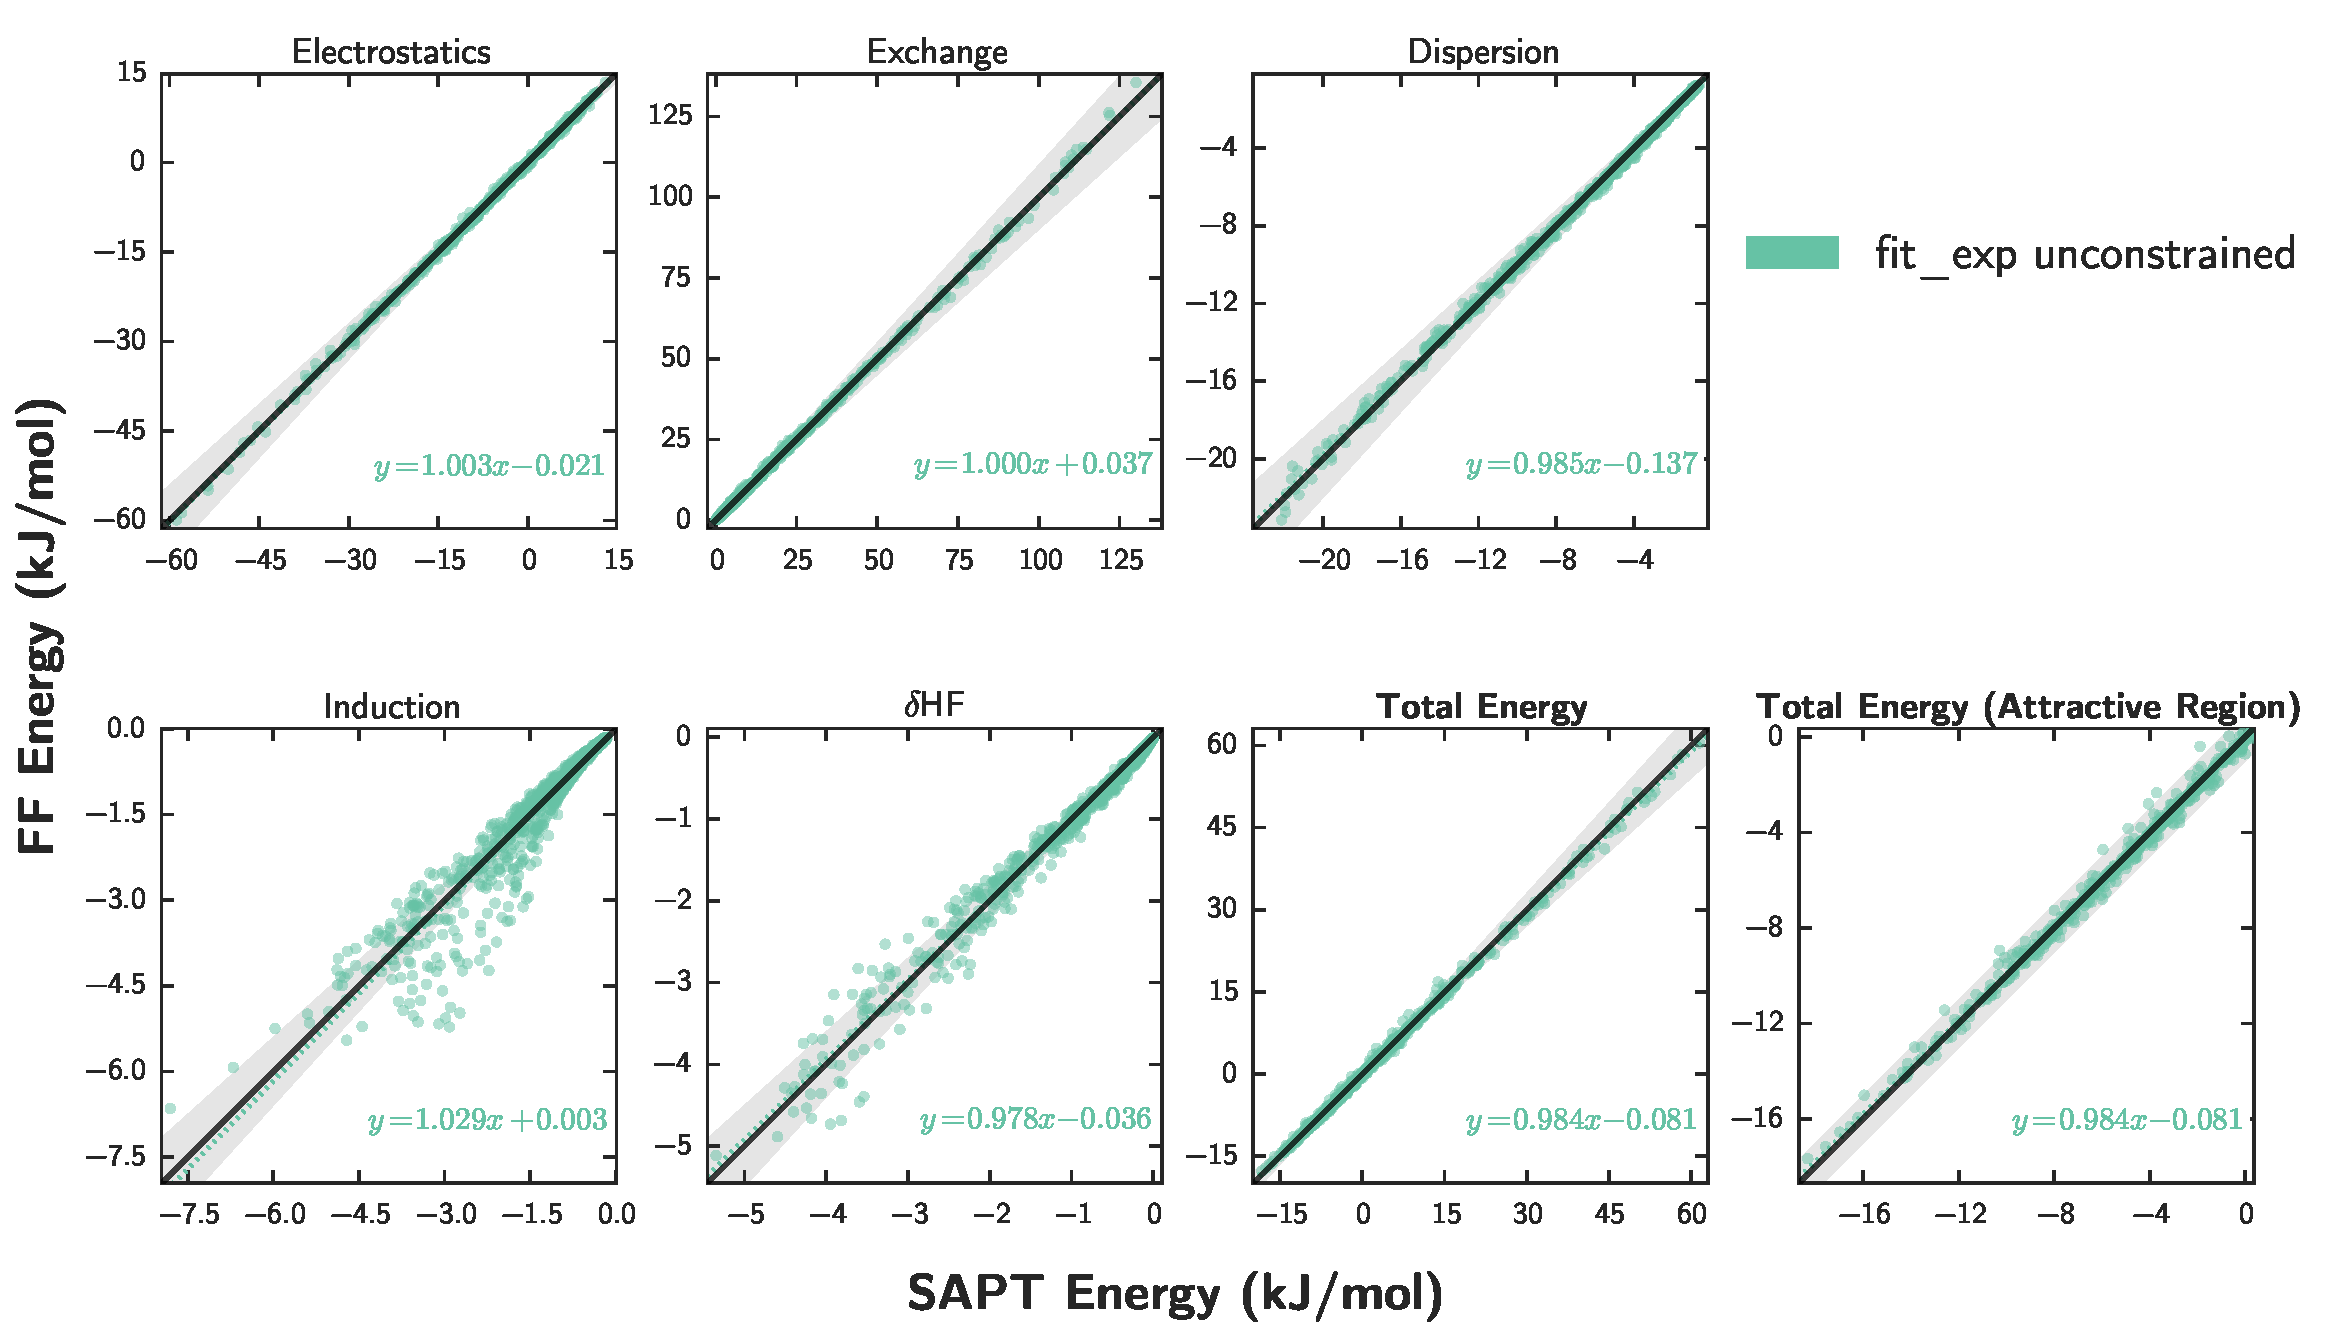
\includegraphics[width=\textwidth]{pointer/water/sapt_comparison.pdf}
\caption[Comparison with the water dimer]
{The water dimer}
\label{fig:pointer-water_fits}
\end{figure}


\begin{figure}
\centering
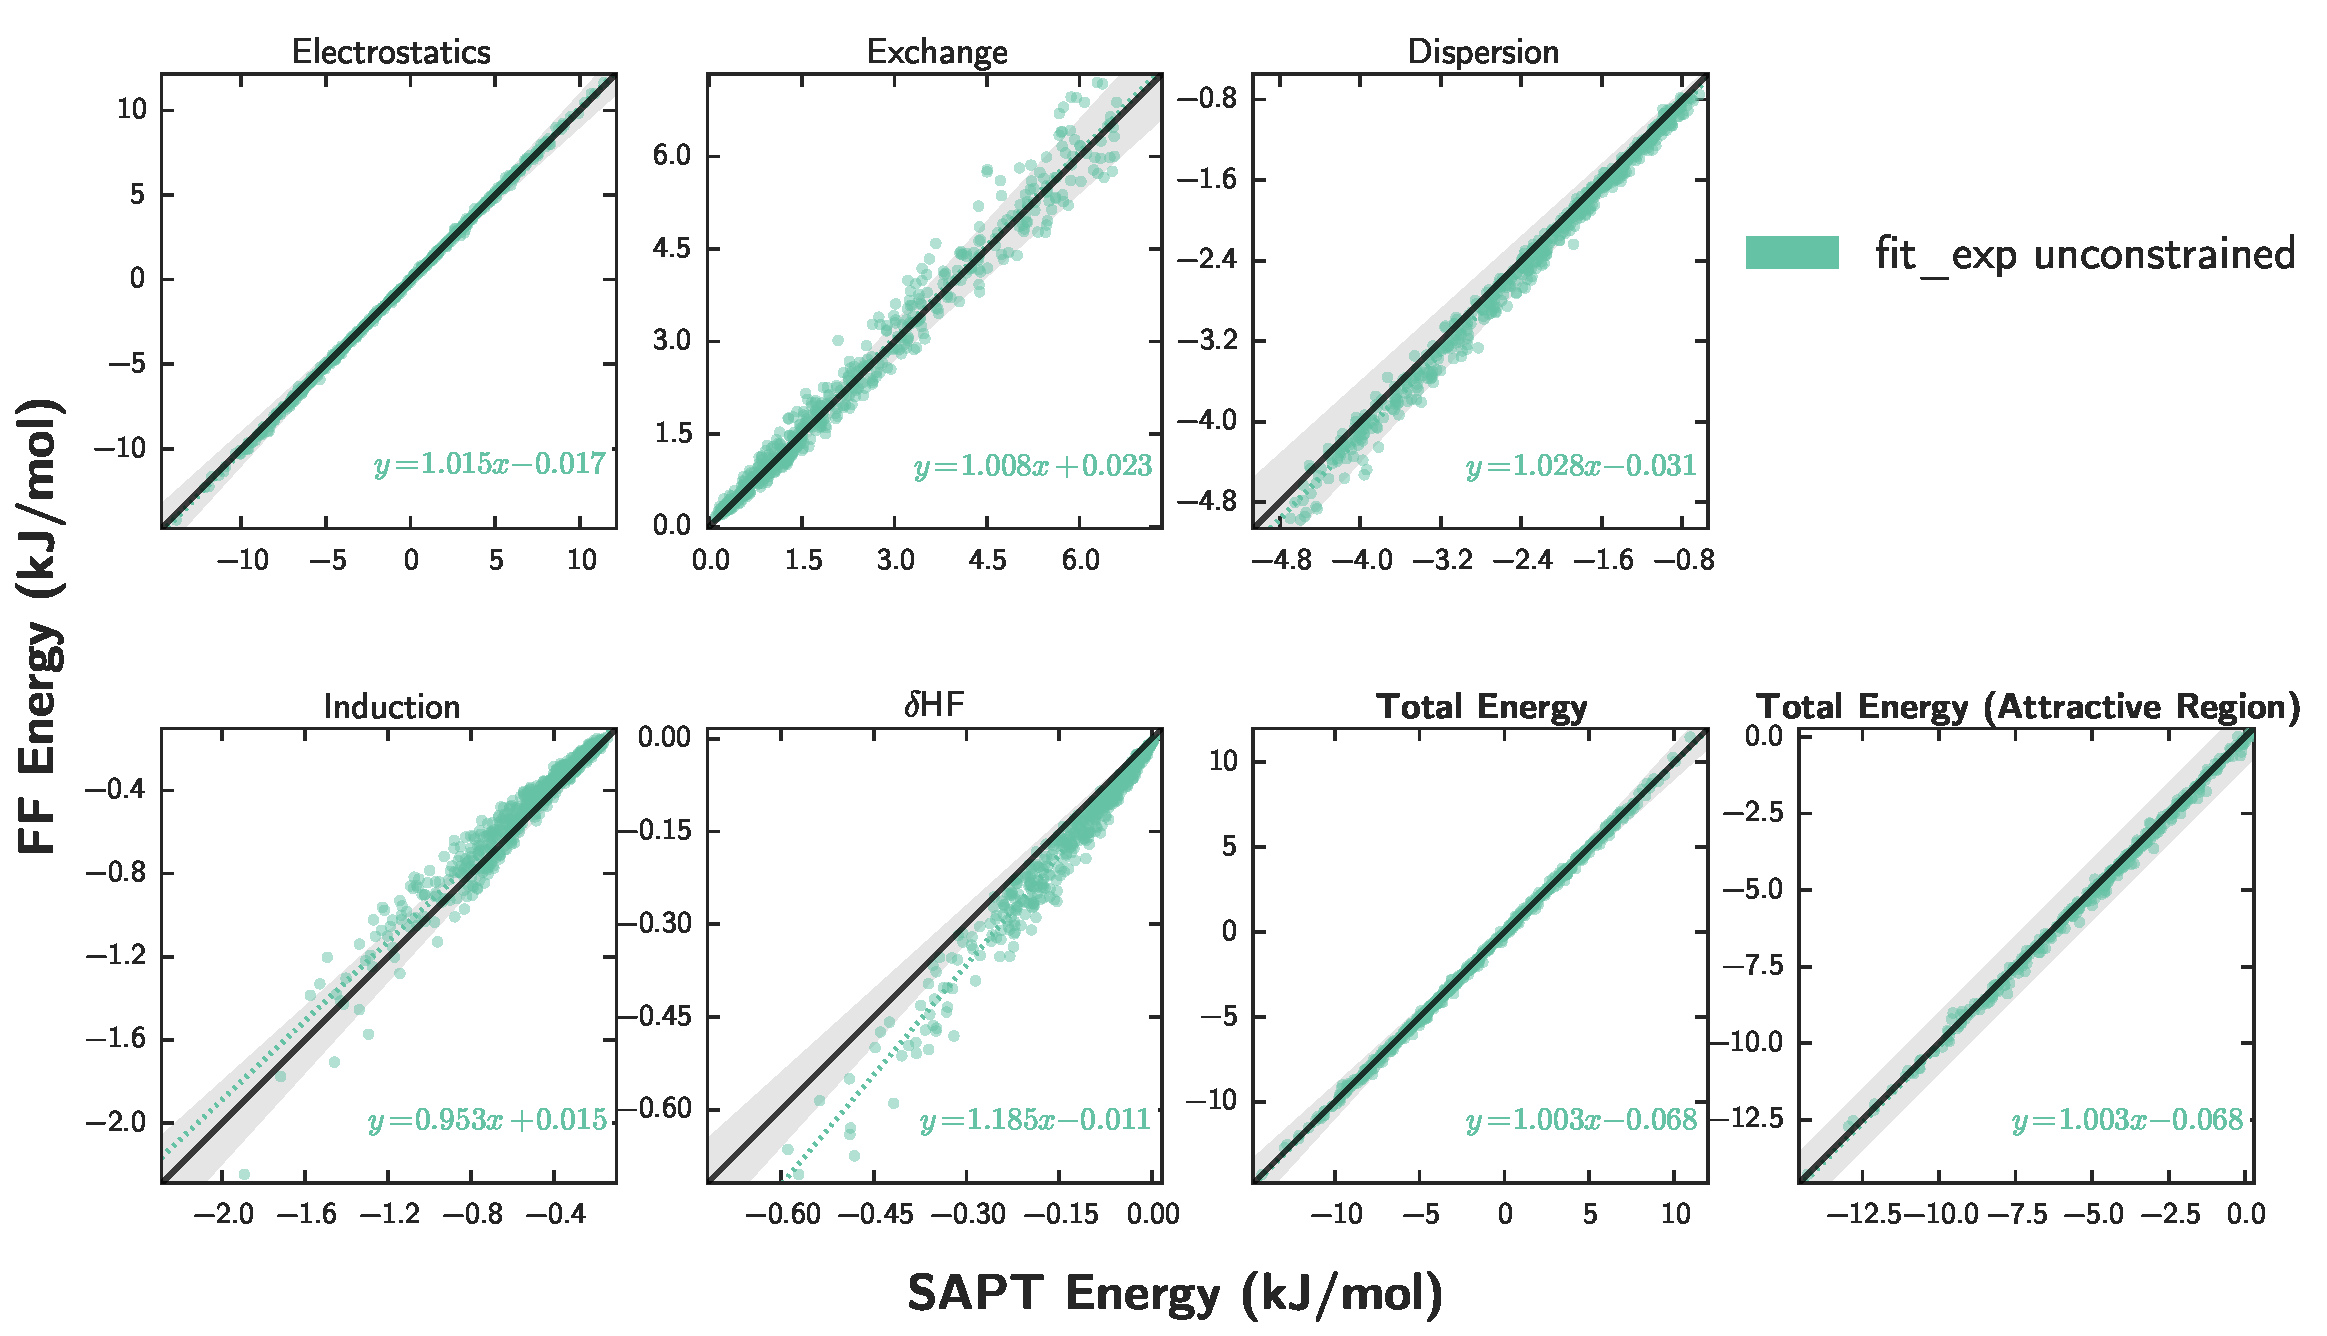
\includegraphics[width=\textwidth]{pointer/water/asymptotic_sapt_comparison.pdf}
\caption[Comparison with the water dimer]
{The water dimer}
\label{fig:pointer-asymptotic_water_fits}
\end{figure}

\begin{figure}
\centering
\fbox{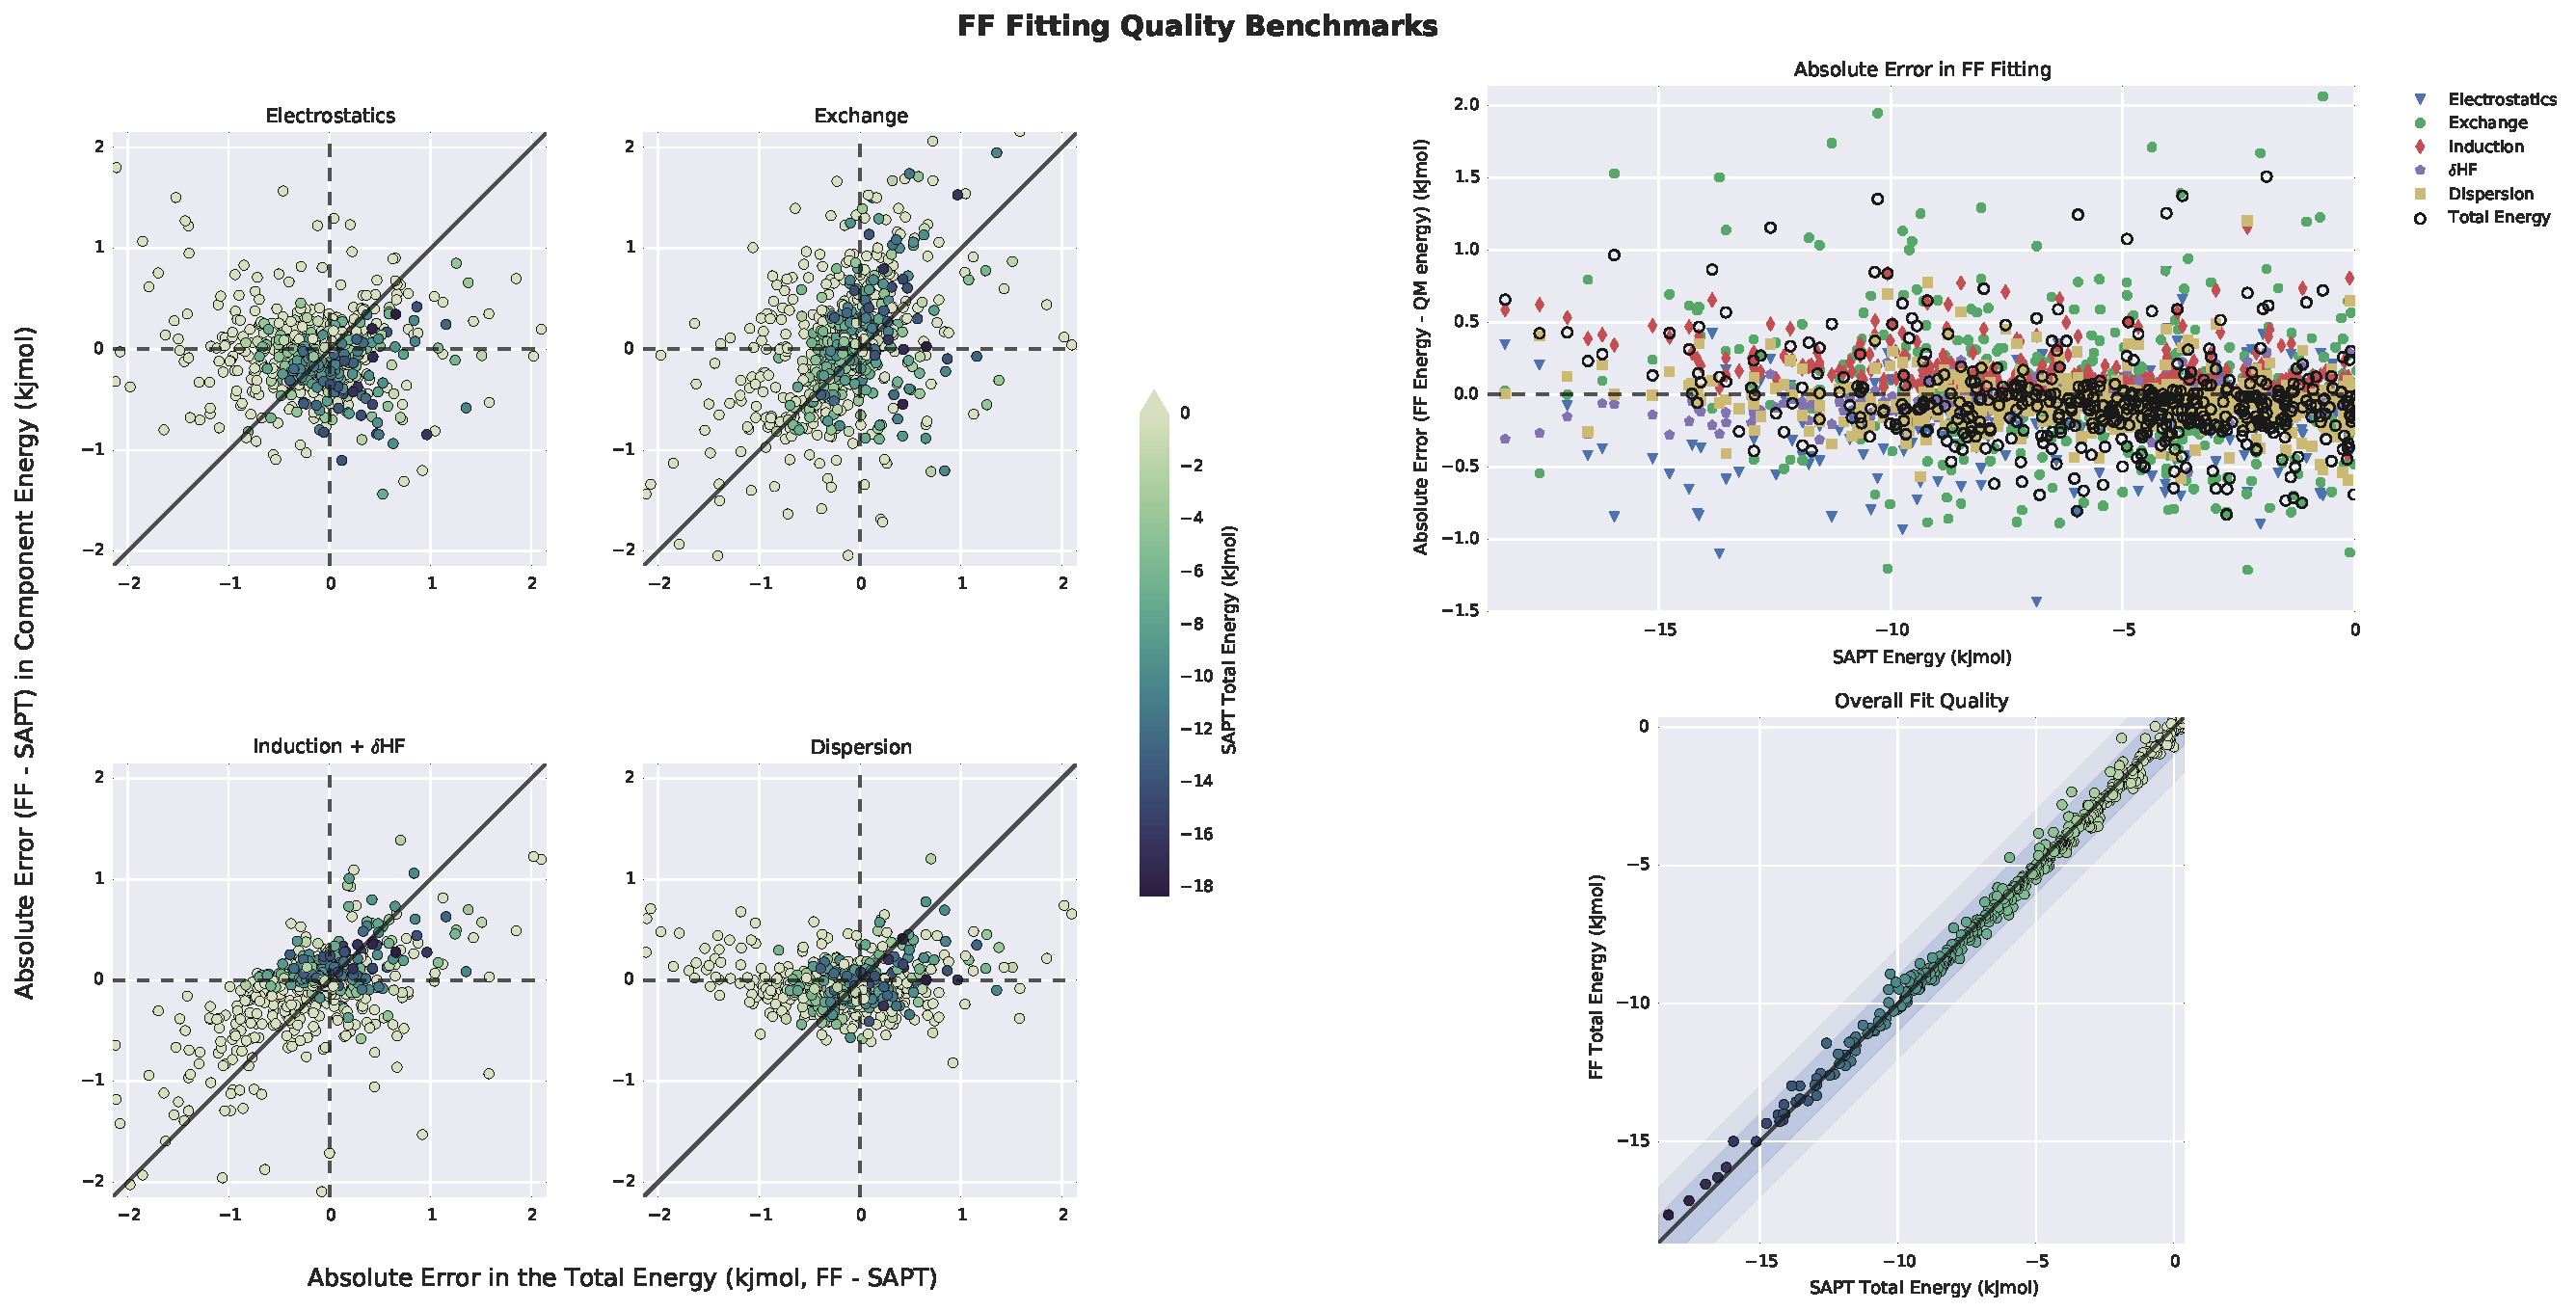
\includegraphics[width=\textwidth]{pointer/water/fit_exp_sapt_errors.pdf}}
\caption[Errors with the water dimer]
{The water dimer errors}
\label{fig:pointer-water_errors}
\end{figure}

\end{paragraph}


\begin{paragraph}{Error Analysis of the Minimum Energy Region}

As discussed in \cref{sec:workflow-geometries}, the mimimum energy region
plays a highly important role in simulations, and thus it is crucial that our
force fields correctly predict these energies. Ideally, the energy predictions
should be within \kjmol{$\pm 1$} of the benchmark energy, though larger errors
are easily possible when developing isotropic force fields. Even more
important than this precision, we must ensure that \emph{on average} the force
field energies are accurate in the minimum energy region. Any systematic
errors in the force field will have a pronounced effect on simulation quality,
particularly for studying bulk properties (as these primarily depend on system
energy averages). 

\cref{fig:pointer-pyridine_errors,fig:pointer-water_errors} show errors in the minimum
energy region for both pyridine and water, and serve as illustrative examples.
These examples have been chosen because both force fields are relatively good quality, but also show errors that could
degrade simulation quality and be the focus of future improvement. 

In the case of pyridine, the force field fit shows fairly little systematic
error, and could probably be used to simulate bulk properties without issue.
Random errors on the order of \kjmol(0.5--1.0) are typical for this force
field, which may or may not be an issue depending on the desired accuracy
level and types of simulations one intends to run. 
(A few outliers show large errors compared to the
\sapt benchmark, however these points almost certainly reside along the
repulsive wall, judging by their exchange energies, and are thus not cause for
great concern.)
If one desired to improve
the precision of the pyridine force field, it is necessary to assess errors in
the force field on a component-by-component basis. \cref{fig:pointer-pyridine_errors}
shows how errors in the exchange component dominate the overall
error, and should be the first target for improvement. Since the exchange energy
only depends on a short-range exponential decay, this error could possibly be
mitigated by increasing the number of atomtypes (right now this force field
only has three atomtypes) or by including anisotropy on additional atomtypes
(right now the potential only includes anisotropy on the nitrogen atom, though
anisotropy in the carbon atoms is almost certainly important).

As for water, we see relatively little random error in the force field
(especially compared to the more isotropic models discussed in
\cref{ch:mastiff}), although again much of this random error can be attributed
to the exchange energy. In contrast to pyridine, however, we see some evidence
for systematic error in the water potential near the minimum energy
configurations. (Indeed, after testing our water force field against the
larger CC-pol database,\cite{Babin2013} we've again found evidence for
overly-repulsive predictions in the minimum energy region.) This systematic
error, small as it may seem, is exacerbated in modeling larger clusters (vida
infra), and would need to be fixed before we could expect good success with
this force field in general water simulations. Looking at the errors on a
component-by-component basis, we can see that systematic errors in the potential
are heavily correlated with errors in the induction energy, making this
induction energy the most important target for improved modeling. As will be
discussed in \cref{ch:future}, improving our polarization model (both in terms
of the polarization damping and the long-range polarizabilities themselves)
will hopefully serve to reduce these systematic errors and improve the overall
quality of our water force field.

\end{paragraph}

\begin{paragraph}{Error Analysis of the Asymptotic Region}

In addition to the minimum energy region, it is important to ensure that the
asymptotic region of the potential is modeled correctly for each energy
component. This asymptotic analysis is shown for the water dimer in
\cref{fig:pointer-asymptotic_water_fits}, where we have shown force field fits
for each component, but have excluded configurations with exchange energies
above a certain threshold. (In general, the magnitude of the \sapt exchange
energy can be used as a proxy for the `short-rangeness' of a given
configuration.) 

Particularly for force fields that directly optimize the dispersion energy, it
is important to ensure that each energy component displays
asymptotically-correct behavior. This analysis can also be used to determine
optimal scaling values for the dispersion coefficients (see
\cref{sec:workflow-dispersion} for details).
\end{paragraph}


\end{subsection}
\begin{subsection}{Validation}

\begin{paragraph}{Trimer Configurations}

Currently, it is hard to guarantee that our polarization models will
correctly describe both the two- and three-body polarization energies. In
order to validate the many-body portion of the potential, trimer
energies should be computed for a subset of energetically-important configurations
(preferably those taken from simulation) and compared to an accurate
electronic structure benchmark. These validation studies are especially
critical for highly-polar systems (such as water), as in these cases the
many-body polarization energy can account for a non-negligable fraction of the
total system energy.

\end{paragraph}

\begin{paragraph}{Simulations}

As the ultimate goal for many potentials is to be able to perform molecular
simulations, it is useful to validate new force field parameters in relation
to `simple' experimental properties. A reasonable starting point for such
comparisons is with the temperature-dependent 2\super{nd} virial coefficient, as this quantity is a
direct measure of the underlying two-body potential. Methods for calculating
the 2\super{nd} virial coefficient are discussed in \cref{ch:isaff,ch:mastiff}
and in \citens{Yu2011,McDaniel2013}.

In addition to the virial coefficient, a variety of other simulations form
useful comparisons to experiment (especially for studying bulk properties),
and examples of these can be found in 
\cref{ch:isaff,ch:mastiff} and in \citens{Yu2011,McDaniel2013,McDaniel2014}.

\end{paragraph}


\end{subsection}
